\section{\texttt{PaasPopCoin}}

The private security and event organization company HSG from the Netherlands wants to build an application (\texttt{PaasPopCoin}) that handles the coin emission and transactions in 
the scope of a medium-size music festival they are organizing. The goal of the system is to allow festival-goers and operators to spend an allotted amount of money in 
relative safety and without the need to bring wallets and other assets around the event. The software in question needs to handle at least three scenarios:
\begin{itemize}
    \item Emission of coins in exchange for money through appropriate cashier desks and ATMs.
    \item Cash-back, that is, exchange of coins with cash in the same locations (we assume that people at the festival may be willing to receive back the money corresponding
        to the coins they have not used).
    \item Tracking of coin expenditure transactions at the various festival shops.
\end{itemize}
In the scope of the above scenarios, there are several special conditions to be considered. First, in the scope of coin emissions, there exist four classes of coin buyers: 
\begin{itemize}
    \item [a.] VIPs who receive a $30\%$ discount on the coins they buy. 
    \item [b.] Event organization people who receive a $50\%$ discount. 
    \item [c.] Event ticket holders class A, who receive a $20\%$ discount. 
    \item [d.] Regular ticket holders who receive no discount.
\end{itemize}
When buying coins, users first need to authenticate themselves by inserting their own ID card in the ATM or by giving it to the cashier; this allows the system to determine 
the class to which each coin buyer belongs. After authentication, buyers get the coins upon inserting into the ATM or giving to the cashier the corresponding amount of money.
Second, also in the context of cash-back, users need to authenticate with their ID card to make sure the appropriate amount of money is given back, considering their role and 
privileges. Third, during the event, every shop clerk keeps track through the \texttt{PaasPopCoin} system of the sales of products and the coins received. \texttt{PaasPopCoin} relies on a 
third-party analytics service to periodically check whether the festival is earning money or not (cost-benefit analysis). Such check is performed with respect to costs of 
products being sold during the event, as well as the overhead to cover all event organization and management expenses. 
\begin{enumerate}
    \item With reference to the Jackson-Zave distinction between the world and the machine, identify the relevant world phenomena for \texttt{PaasPopCoin}, including the ones shared 
        with the machine, providing a short description if necessary. For shared phenomena specify whether they are controlled by the world or the machine. Focus on phenomena 
        that are relevant to describe the requirements of the system.
    \item Describe through a UML Class Diagram the main elements of the \texttt{PaasPopCoin} domain. 
    \item Define a UML Use Case Diagram describing the relevant actors and use cases for \texttt{PaasPopCoin}. 
        You can provide a brief explanation of the Use Case Diagram, especially if the names of the use cases are not self-explanatory.
\end{enumerate}

\paragraph*{Solution}
\begin{enumerate}
    \item The world-only phenomena can be: 
        \begin{itemize}
            \item User buys Class A ticket.
            \item User buys regular ticket.
            \item VIP is contracted for event.
            \item Event organization is started and contractors registered.
            \item Event starts.
            \item User gives money to cashier (to be converted in coins).
            \item User gives coins to cashier (to be converted in money).
            \item User gives ID card to cashier.
            \item User buys some product at festival.
            \item The external analytics service checks the success of an event.
        \end{itemize}

        The shared phenomena can be the following: 
        \begin{itemize}
            \item User inserts money into an ATM.
            \item ID Card is inserted into ATM.
            \item User inserts coins into an ATM.
            \item Cashier inserts in the system an ID card number.
            \item Cashier inserts in the system the amount of money handed by a certain user.
            \item Cashier inserts in the system the amount of coins returned by a certain user.
            \item Store clerk inputs in system the amount of coins spent by user in shop.
            \item The system enables coin emission after checking ID card and inserted amount of money.
            \item The system enables cash-back after checking ID card and inserted number of coins.
            \item The system sends data about purchases to the external analytics service.
        \end{itemize}
    \item The UML diagram of the given problem is: 
        \begin{figure}[H]
            \centering
            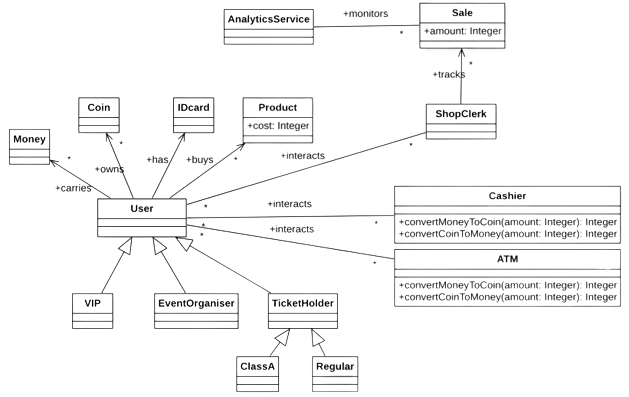
\includegraphics[width=0.9\linewidth]{images/UML.png}
        \end{figure}
    \item The UML use case diagram of the given problem is: 
        \begin{figure}[H]
            \centering
            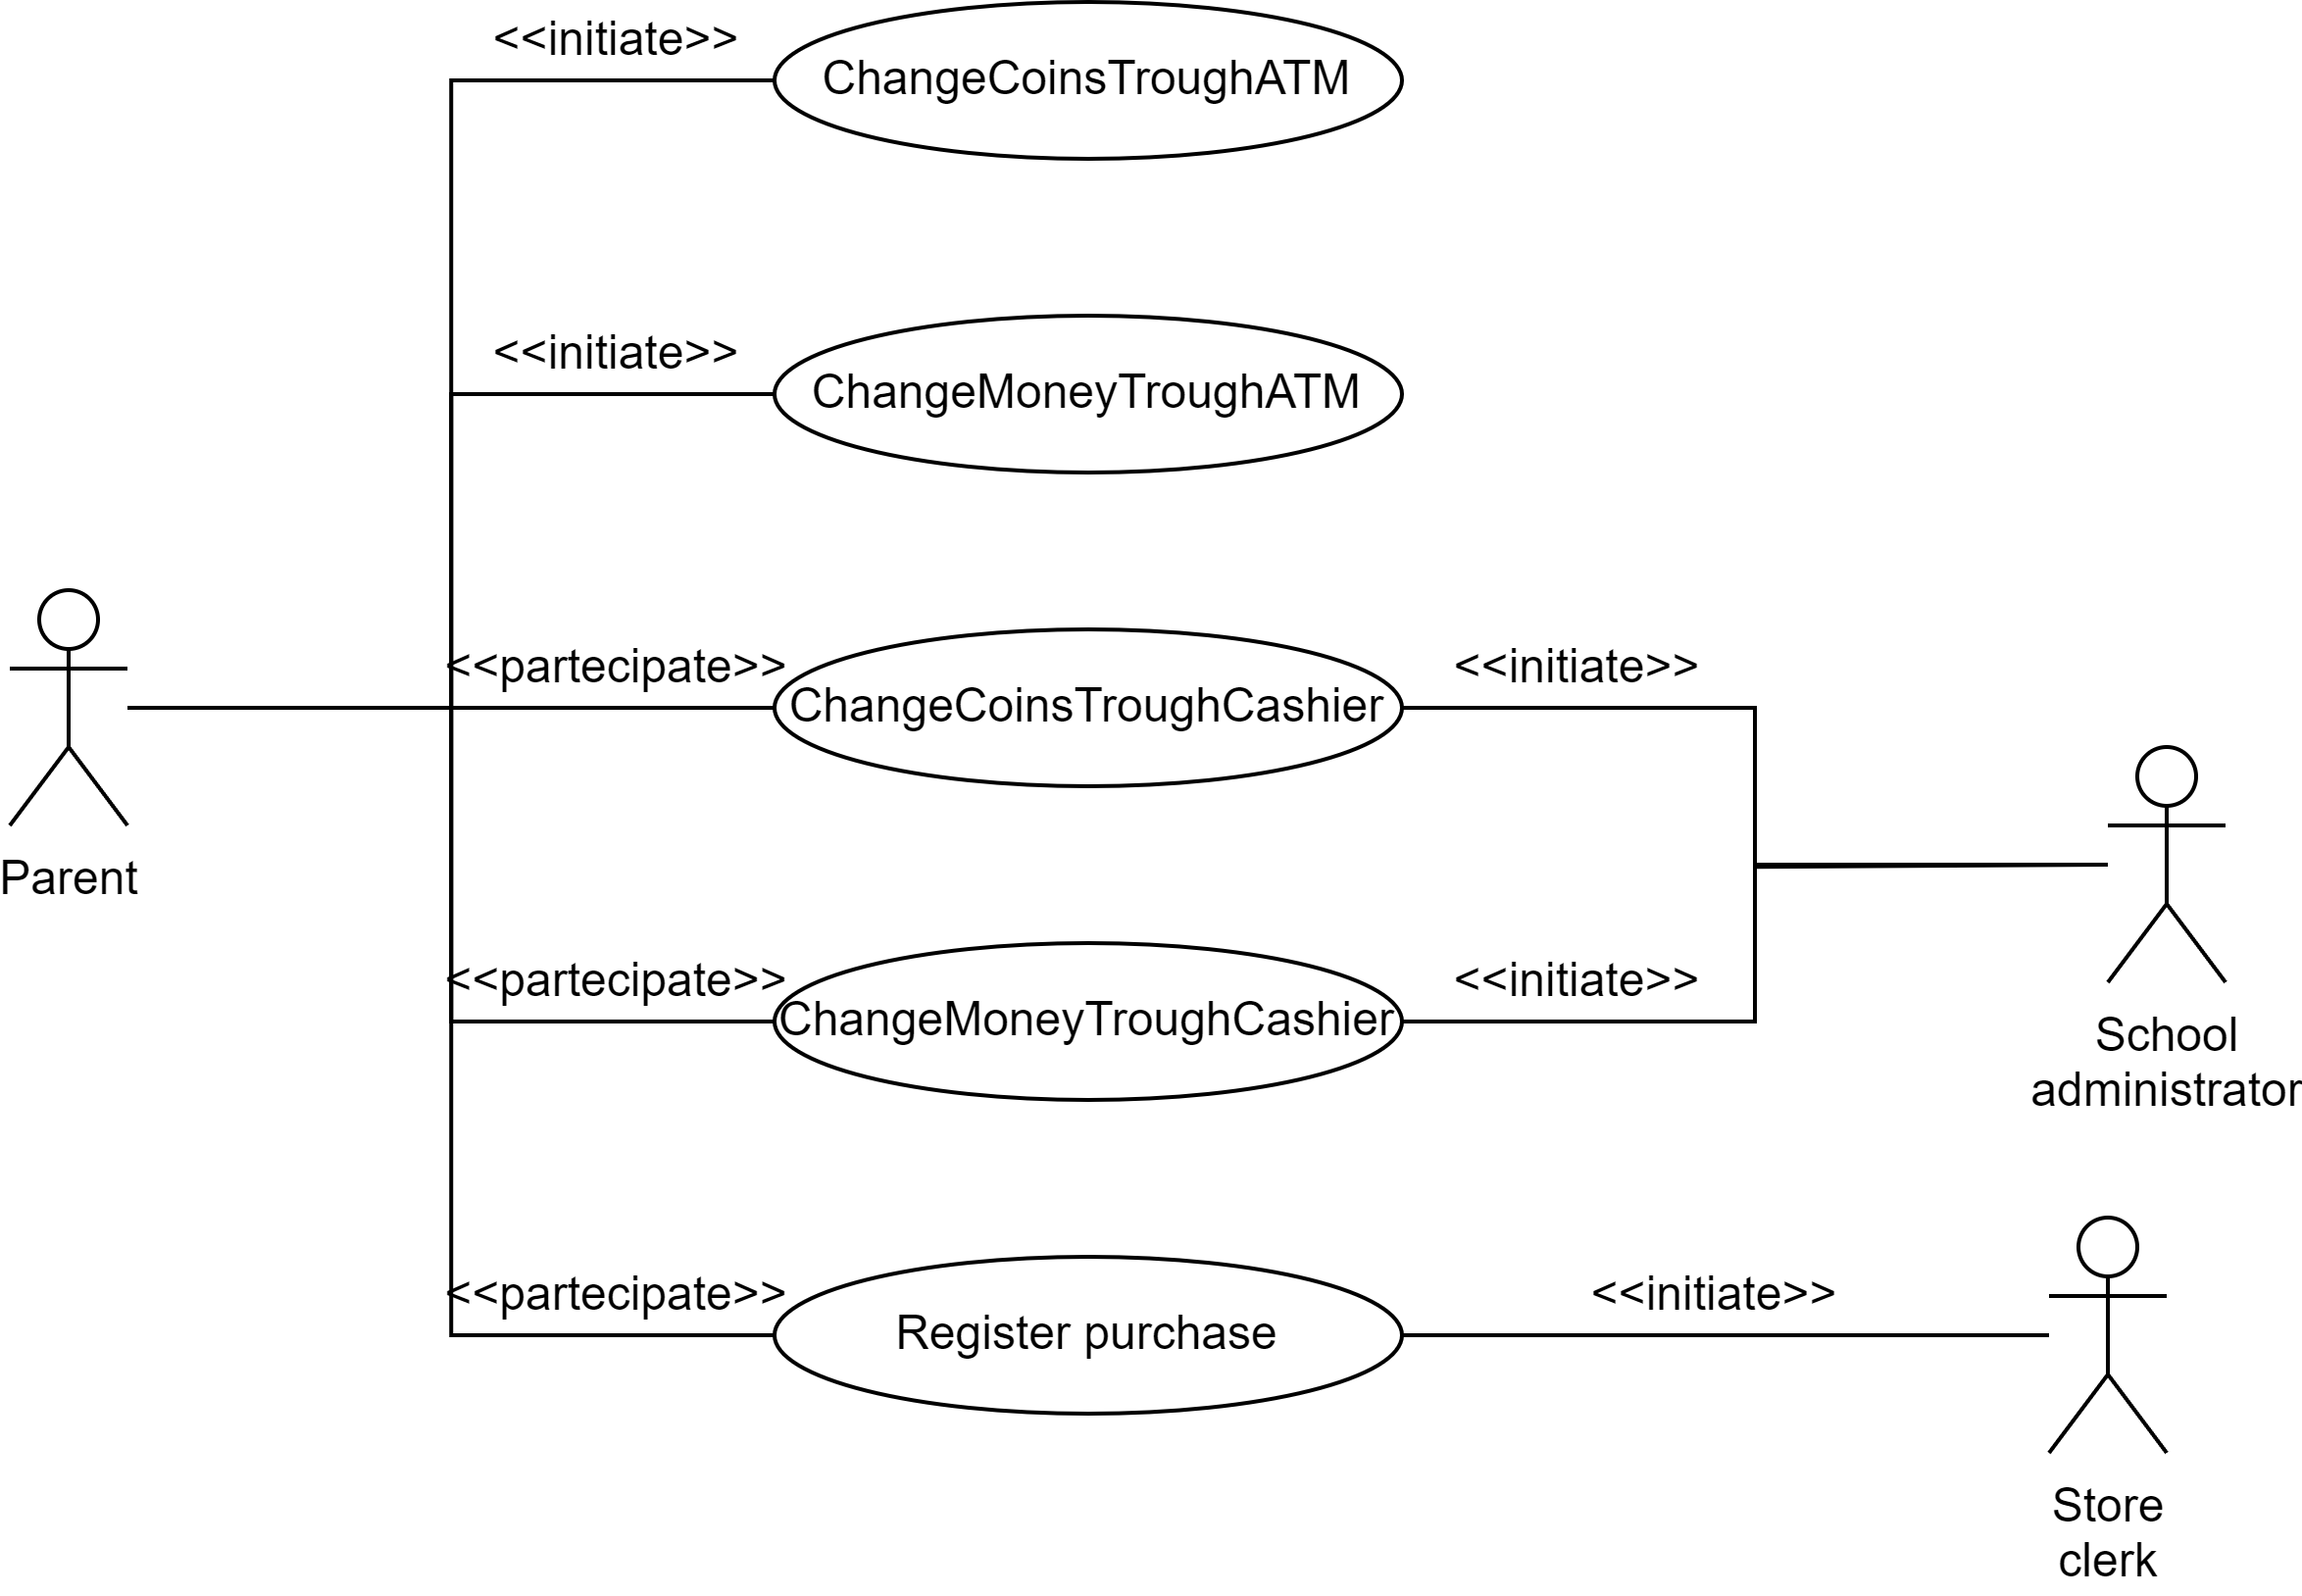
\includegraphics[width=0.9\linewidth]{images/usecase2.png}
        \end{figure}
\end{enumerate}